\section{The Numerical Renormalization Group Approach}

Now that we have understood the qualitative picture of what the physics looks like, we can being to discuss the NRG proposed by Wilson which finally yielded correct results at low energies. We start, first, with some generic information about what the renormalization group is, then we will get into Wilson's application of it to the Kondo problem.

\subsection{The Renormalization Group}\label{sec:5-nrg-renormgroup}

In the most general way, the renormalization group is a mapping of one Hamiltonian consisting of one set of parameters to a Hamiltonian of the same form with a ``renormalized'' set of parameters, valid at a new energy scale. Denoting the original set of parameters as $\vv{K}$ and the renormalized as $\vv{K}'$, we can write this as:

\begin{equation}
  \mathcal{R}_\alpha[\hat{H}(\vv{K})] = \hat{H}(\vv{K}'),
\end{equation}

or equivalently:

\begin{equation}
  \mathcal{R}_\alpha(\vv{K}) = \vv{K}'.
\end{equation}

This renormalization is characterized by a parameter $\alpha$ which is related to the ratio of the energy scales between the two sets of parameters. Applying many subsequent transformations forms a \textit{trajectory} for the parameters. In this application, this is done by reducing the energy scale for successive transformations.

A \textit{fixed point} in parameter space is a set of parameters $\vv{K}^*$ which remains invariant under a renormalization group transformation; i.e. it maps the Hamiltonian onto itself:

\begin{equation}
  \mathcal{R}[\hat{H}(\vv{K}^*)] = \hat{H}(\vv{K}^*).
\end{equation}

We can linearize the transformation (which is otherwise, in general, not linear) around this fixed point for some $\vv{K} = \vv{K}^* + \delta\vv{K}$, after which we can expand around the fixed point:

\begin{equation}
  \mathcal{R}_\alpha(\vv{K}^* + \delta\vv{K}) = \vv{K}^* + \vv{L}^*_\alpha\delta\vv{K} + \mathcal{O}(\delta\vv{K}^2).
\end{equation}

From here, if we know the eigenvectors and eigenvalues of $\vv{L}_\alpha^*$ and make the assumption that they are complete, they can be used as a basis for $\delta\vv{K}$. Then, we are able to write (discarding higher order contributions) an equation for the application of $\mathcal{R}_\alpha$ on the region around the fixed point:

\begin{equation}
  \mathcal{R}_\alpha(\vv{K}^* + \delta\vv{K}) = \vv{K}^* + \sum_n (\delta K)_n \lambda^*_n \vv{E}^*_n,
\end{equation}

where $(\delta K)_n$ are the components of $\delta\vv{K}$, and $\lambda^*_n$ and $\vv{E}^*_n$ are the eigenvectors and eigenvalues of $\vv{L}^*$. In general, this transformation can be applied $m$ times:

\begin{equation}
  \mathcal{R}^m_\alpha(\vv{K}^* + \delta\vv{K}) = \vv{K}^* + \sum_n (\delta K)_n (\lambda^*_n)^m \vv{E}^*_n,
\end{equation}

There are different classifications for the values that the eigenvalues can take, but their names are not particularly relevent for the scope of this project. What is important, though, is the fact that we are able to describe the behavior in a region around the fixed point by using the effective Hamiltonian for that fixed point. Anderson's poor man's scaling approach was essentially done in this way by successively reducing the energy scale of the conduction band -- the parameter $\alpha$ would relate the successive energy scales. His set of parameters consisted only of the coupling $J$ between the impurity spin and the conduction electron spins. In the antiferromagnetic case, we can notice that $J \rightarrow \infty$ is one such fixed point. Our goal (Wilson's goal, rather), then, phrased in terms of the Anderson model, is to apply this approach such that we determine the effective Hamiltonian for this fixed point. We can then use this effective Hamiltonian to determine behavior near the fixed point, and then make calculations of thermodyamic quantities such as the resistivity.

In principle, we are able to determine the exact forms of these effective Hamiltonians, from which we can make these additional calculations. I was unable to fully explore this side of things, but found it valuable to describe fixed points and effective Hamiltonians because they are the means by which the results are calculated with higher accuracy. The renormalization group method itself, as we will see, is still very effective, but does carry some error as its starting point is a Hamiltonian effective at a much higher energy scale (that being whatever the initial energy scale is chosen to be for the evolution). It is then progressively rescaled, but still retains its original form. Again, this works very well: however by determining the exact form of the effective Hamiltonians at the $J\rightarrow\infty$ fixed point would, in principle, let us make more accurate calculations.


\subsection{The Numerical Renormalization Group}

With this, we can now explore the main part of this project: the NRG. It is worth pointing out, though, that this method is highly specialized to this application, i.e. the Anderson impurity model --  it is an immensely challenging problem and thus some generic methods just simply don't work. With this, the general steps for the NRG procedure are:

\begin{figure}
  \centering
  \begin{subfigure}[b]{0.3\linewidth}
    \centering
    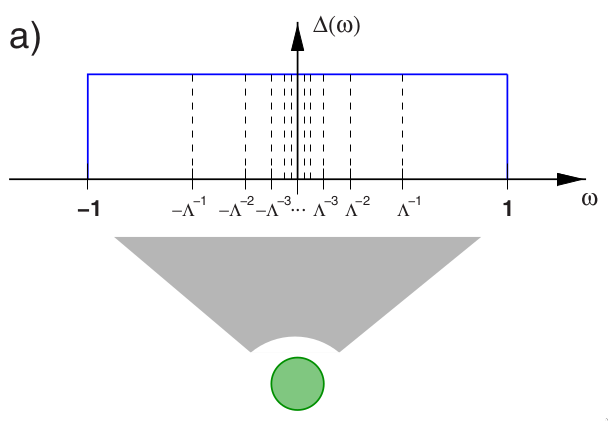
\includegraphics[width=\linewidth]{./gfx/nrg-a.png}
    \caption{Logarithmic binning.}
    \label{fig:4-nrg-schematics-a}
  \end{subfigure}
  \begin{subfigure}[b]{0.3\linewidth}
    \centering
    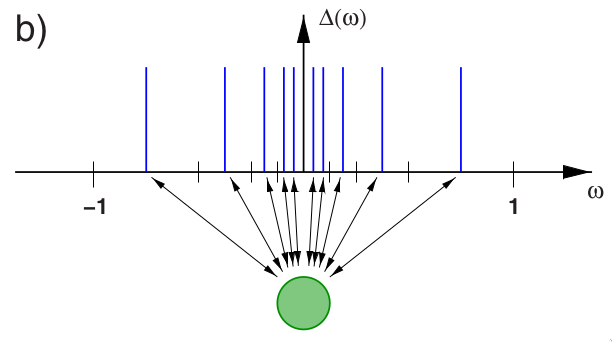
\includegraphics[width=\linewidth]{./gfx/nrg-b.png}
    \caption{Discretization.}
    \label{fig:4-nrg-schematics-b}
  \end{subfigure}
  \begin{subfigure}[b]{0.3\linewidth}
    \centering
    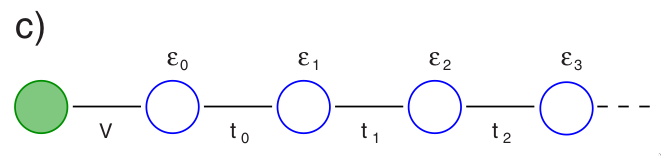
\includegraphics[width=\linewidth]{./gfx/nrg-c.png}
    \caption{Mapping to linear chain.}
    \label{fig:4-nrg-schematics-c}
  \end{subfigure}
  \caption{Diagrammatical representation of the main steps involved in the NRG procedure.}
  \label{fig:4-nrg-schematics}
\end{figure}

\begin{enumerate}
\item Divide the energy spectrum into logarithmic bins via a parameter $\Lambda > 1$, giving positive and negative energy intervals $[\Lambda^{-(n+1)},\lambda^{-n}]$ and $[-\Lambda^{-n},-\lambda^{-(n+1)}]$, as in Fig.~\ref{fig:4-nrg-schematics-a}.
\item Pick a single characteristic state from within each continuous interval, such that we have a discrete set of states (separated logarithmically), as in Fig.~\ref{fig:4-nrg-schematics-b}.
\item Map these continuous states onto a semi-infinite linear chain with the impurity site placed at one end, as in Fig.~\ref{fig:4-nrg-schematics-c}.
\item Iteratively diagonalize the resulting Hamiltonian after adding subsequent conduction sites to the end of the linear chain.
\end{enumerate}



The reason as to why we are doing it this way, i.e. ultimately mapping onto a chain, is because of the fact that adding subsequent sites is a relatively easy thing to do computationally as it is inherently iterative. Further, as we will see later on, we can utilize symmetries of the problem in order to reduce the size of the matrices that we have to diagonalize, since they would in principle grow exponentially based on the dimension of the added basis of the new site. This makes their computation significantly easier, rendering this technique very useful.

One question that may be asked is how this pertains to a renormalization group transformation at each step. In particular, our goal is to resolve the low energy behavior of our system further and further each iteration, leaving us with an effective Hamiltonian valid at each new energy scale. The iterative step involves adding a new site to the end of the chain, which interacts with the one before it via the hopping term $t_n$. As we will find out, the logarithmic discretization leads to these terms being proportional to $\Lambda^{-n/2}$. Therefore, the interpretation of the added site is that we are accessing an new energy scale that is reduced by a factor of $\sqrt{\Lambda}$. This is the essence of the NRG; it will be reiterated once we have all the pieces.



\subsubsection{Logarithmic Discretization}

To reiterate, Anderson's model describes the impurity as a localized moment formed by a Coulomb interaction $U$ between two electrons. The total Hamiltonian, including the sum of the contributions from the impurity, the bath, and the interaction between the two is given by\footnote{Note the change of notation here compared to that in Sec.~\ref{sec:3-variational}; the creation/annihilation operators for the $d$-level of the impurity are now represented by $f$s. This is to reflect what is seen in the literature and code documentation. Also, in principle, it is the $f$-orbitals in heavy fermions which are more strongly interacting.}

\begin{align}
  \hat{H} &= \hat{H}_{\text{imp}} + \hat{H}_{\text{bath}} + \hat{H}_{\text{int}} \\
          &= \sum_\sigma \epsilon_f \hat{f}^\dagger_\sigma \hat{f}_\sigma + U\hat{f}^\dagger_\uparrow \hat{f}_\uparrow \hat{f}^\dagger_\downarrow \hat{f}_\downarrow + \sum_{k,\sigma}\epsilon_k \hat{c}^\dagger_{k\sigma}\hat{c}_{k\sigma} + \sum_{k,\sigma}V_k(\hat{f}^\dagger_\sigma \hat{c}_{k,\sigma} + h.c.),
\end{align}

where the $f$ operators create impurity states with energy $\epsilon_f$, the $c$ operators create bath states with energies $\epsilon_k$, and $V_k$ is a hybridization term. (Hats will be dropped from operators from here on out.) The physical quantity related to the influence of the bath of conduction states on the impurity is determined by the \textit{hybridization function} $\Delta(\omega)$, given by

\begin{equation}
  \Delta(\omega) = \pi\sum_k V_k^2 \delta(\omega - \epsilon_k).
\end{equation}

Since this is a \textit{physical} quantity, we want to ensure that its form remains the same after doing the following transformations. One such transformation that we can do is to bring the bath and interaction components into the continuum:

\begin{equation}
  \hat{H} = \hat{H}_{\mathrm{imp}} + \sum_\sigma \int_{-1}^1 \dd\epsilon \; g(\epsilon) a^\dagger_{\epsilon\sigma}a_{\epsilon\sigma} + \sum_\sigma \int_{-1}^1 \dd\epsilon \; h(\epsilon)(f^\dagger_\sigma a_{\epsilon\sigma} + a^\dagger_{\epsilon\sigma}f_{\sigma}),\label{eq:continuous-hamiltonian}
\end{equation}

with $g(\epsilon)$ being the dispersion and $h(\epsilon)$ being the hybridization, which are now continuous. These new $a$ operators satisfy standard fermionic commutation relations, and we have also imposed energy cutoffs at $\epsilon=\pm1$ (i.e. by imposing a bandwidth of $[-1,1]$).

We may now define our parameter $\Lambda$, which will serve to discretize our energy spectrum:

\begin{equation}
  x_n = \pm\Lambda^{-n}, \quad n=0,1,2,\ldots,
\end{equation}

with the width of each interval determined by

\begin{equation}
  d_n = \Lambda^{-n}(1 - \Lambda^{-1}).
\end{equation}

Of course, we must have $\Lambda > 1$. Inside of each interval, we can now define a complete set of orthonormal functions which are simply plane waves with characteristic frequency determined simply by $\omega_n = 2\pi/d_n$ (and normalized to the interval width):

\begin{equation}
  \psi^\pm_{np}(\epsilon) =
  \begin{alignedat}{1}
    \begin{cases}
      \frac{1}{\sqrt{d_n}}e^{\pm i\omega_n p\epsilon}, \quad & \text{for}\ x_{n+1} < \epsilon < x_n,\ \text{and} \\
      0 & \text{otherwise},
    \end{cases}
  \end{alignedat}
\end{equation}

where $p \in \mathbb{Z}$. We can expand the original $a$ operators in this new basis like so:

\begin{equation}
  a_{\epsilon\sigma} = \sum_{np}\left(a_{np\sigma}\psi^+_{np}(\epsilon) + b_{np\sigma}\psi^-_{np}(\epsilon)\right),
\end{equation}

At this point, by using the $a_{\epsilon,\sigma}$ operators, we now have expressed our Hamiltonian from Eq.~\eqref{eq:continuous-hamiltonian} in terms of discrete creation and annihilation operators for states residing within each logarithmic band. To assist with notation for the following steps, we define:

\begin{equation}
  \int^{+n}\dd\epsilon \equiv \int_{x_{n+1}}^{x_n}\dd\epsilon, \quad\text{and}\quad \int^{-n}\dd\epsilon \equiv \int_{-x_n}^{-x_{n+1}}\dd\epsilon.
\end{equation}

With this, we can express the hybridization term of our quasi-continuous Hamiltonian like so:

\begin{equation}
  \int_{-1}^1\dd\epsilon \; h(\epsilon) f^\dagger_\sigma a_{\epsilon\sigma} = f^\dagger_\sigma \sum_{np} \left[ a_{np\sigma}\int^{+n}\dd\epsilon \; h(\epsilon)\psi^+_{np}(\epsilon) + b_{np\sigma}\int^{-n}\dd\epsilon \; h(\epsilon) \psi^-_{np}(\epsilon) \right],
\end{equation}

where the other term will of course just be the conjugate. It is here we make one important assumption: that the hybridization $h(\epsilon)$ remain constant within each band, i.e. that $h(\epsilon) = h$. If we make this assumption, then the above integrals actually filter out only the $p=0$ state:

\begin{equation}
  \int^{\pm n}\dd\epsilon \; \psi^{\pm}_{np}(\epsilon) = \sqrt{d_n}h\delta_{p,0},
\end{equation}

which has the physical implication that the impurity states only couple to the $p=0$ conduction states.\footnote{This relation can be very easily shown using the definition of the basis states.} We could have also imposed this fact instead, which would have led to a constant hybridization. These are equivalent, and they are the defining assumption from Wilson's technique. Now, we can make a further assumption with the hybridization: it is defined as a sort of \textit{step} function where it is equal to the average of the hybridization function over that interval:

\begin{equation}
  h(\epsilon) = h_n^{\pm},\quad x_{n+1} < \pm\epsilon < x_n,
\end{equation}

where

\begin{equation}
  h_n^{\pm 2} = \frac{1}{d_n} \int^{\pm n} \dd\epsilon \; \frac{\Delta(\epsilon)}{\pi}.
\end{equation}

With this in mind, the hybridization term in our Hamiltonian turns out to be:

\begin{equation}
  \int_{-1}^1\dd\epsilon \; h(\epsilon) f^\dagger_{\sigma}a_{\epsilon\sigma} = \frac{1}{\pi}f^\dagger_\sigma \sum_n \left( \gamma^\dagger_n a_{n0\sigma} + \gamma^-_n b_{n0\sigma} \right),
\end{equation}

where the $\gamma$ terms are given by

\begin{equation}
  \gamma^{\pm2}_n = \int^{\pm n}\dd\epsilon \; \Delta(\epsilon).
\end{equation}

We can now do the same for the conduction electron term:

\begin{align}
  \int_{-1}^1 \dd\epsilon \; g(\epsilon) a^\dagger_{\epsilon\sigma}a_{\epsilon\sigma} &= \sum_{np} \left( \xi^+_n a^\dagger_{np\sigma}a_{np\sigma} + \xi^-_n b^\dagger_{np\sigma}b_{np\sigma} \right) \\
                                                                                      &+ \sum_{n,p \neq p'}\left[ \alpha^+_n(p,p')a^\dagger_{np\sigma}a_{np'\sigma} - \alpha^-_n(p,p')b^\dagger_{np\sigma}b_{np'\sigma} \right].\label{eq:cond-elect-exact}
\end{align}

The first term on the right is already diagonal in $p$; it turns out we can hence express the eigenvalues $\xi$ as

\begin{equation}
  \xi^{\pm}_n = \frac{\int^{\pm }\dd\epsilon \; \Delta(\epsilon)\epsilon}{\int^{\pm }\dd\epsilon \; \Delta(\epsilon)}.\label{eq:xi-exact}
\end{equation}

If we assume a constant $\Delta(\epsilon)$, then this simplifies to

\begin{equation}
  \xi^{\pm}_n = \frac{1}{2}\Lambda^{-n}(1 + \Lambda^{-1}) = \frac{d_n}{2}.
\end{equation}

In the case of a linear dispersion term, i.e. $g(\epsilon) = \epsilon$, we can determine the form of the $\alpha$ prefactors in Eq.~\eqref{eq:cond-elect-exact}:

\begin{equation}
  \alpha^{\pm}_n(p,p') = \frac{1 - \Lambda^{-1}}{2\pi i}\frac{\Lambda^{-n}}{p'-p} \exp{\frac{2\pi i(p'-p)}{1 - \Lambda^{-1}}}.
\end{equation}

Here we can make a bit of a better argument for the dropping of $p\neq0$ terms. The $\alpha$ prefactors contain a term like $1-\Lambda^{-1}$, which, in the continuum limit where $\Lambda \rightarrow 1$, will go to zero. It is through these that the $p\neq0$ terms interact with the $p=0$ term. We can hence treat any terms above $p=0$ as a \textit{perturbation} to the $p=0$ term; if we consider just leading order, this involves dropping the $p\neq0$ terms. It may seem like a crude approximation, but it turns out to work very well even for moderately large values of $\Lambda$, such as 2 or 3.\footnote{Most of this section has come from Refs.~\cite{Bulla_2008} and~\cite{Hewson_1993} and isn't particularly groundbreaking, hence the lack of individual citations; this, however, is a bit of a interesting result, so I directly cite these two here for a bit of an exploration on this approximation. Further, Wilson's original paper~\cite{Wilson_1975} contains some commentary on it.}

So, dropping all $p \neq 0$ terms, we will have fully achieved the logarithmic discretization of the Hamiltonian:

\begin{align}
  \hat{H} = \hat{H}_{\mathrm{imp}} &+ \sum_{n\sigma} \left( \xi^+_n a^\dagger_{n\sigma}a_{n\sigma} + \xi^-_n b^\dagger_{n\sigma}b_{n\sigma} \right) \\
          &+ \frac{1}{\sqrt{\pi}}\sum_\sigma f^\dagger_\sigma \sum_n \left( \gamma^+_n a_{n\sigma} + \gamma^-_n b_{n\sigma} \right) \\
          &+ \frac{1}{\sqrt{\pi}} \sum_\sigma \left( \sum_n \left( \gamma^+_n a^\dagger_{n\sigma} + \gamma^-_n b^\dagger_{n\sigma} \right) \right)f_\sigma.
\end{align}


\subsubsection{Mapping to Semi-Infinite Linear Chain}

Our next goal is to map this discretized Hamiltonian onto a semi-infinite chain with the impurity placed at the first site. This means we will have the impurity connected to only a single conduction electron with operators $c^{(\dagger)}_{0\sigma}$, and we will have hopping terms connecting the bath states. We can determine the form of the $c^{(\dagger)}_{0\sigma}$ operators from our final expression for the discretized Hamiltonian:

\begin{equation}
  c_{0\sigma} = \frac{1}{\sqrt{\xi_0}} \sum_n \left( \gamma^+_n a_{n\sigma} + \gamma^-_n b_{n\sigma} \right),
\end{equation}

with normalization

\begin{equation}
  \xi_0 = \sum_n\left[ (\gamma^+_n)^2 + (\gamma^-_n)^2 \right] = \int_{-1}^1 \dd\epsilon \; \Delta(\epsilon).
\end{equation}

In terms of $c_{0\sigma}$, the hybridization term can be written like

\begin{equation}
  \frac{1}{\sqrt{\pi}} f^\dagger_\sigma \sum_n \left( \gamma^+_n a_{n\sigma} + \gamma^-_n b_{n\sigma} \right) = \sqrt{\frac{\xi_0}{\pi}}f^\dagger_\sigma c_{0\sigma},
\end{equation}

and the $c^\dagger_{0\sigma}$ operator follows similarly. After doing this, we find that our chain Hamiltonian looks like:

\begin{equation}
  \hat{H} = \hat{H}_{\mathrm{imp}} + \sqrt{\frac{\xi_0}{\pi}} \sum_\sigma \left( f^\dagger_\sigma c_{0\sigma} + c^\dagger_{0\sigma}f_\sigma \right) = \hat{H}_{\mathrm{imp}} + \sum_{\sigma n=0}^{\infty} \left[ \epsilon_nc^\dagger_{n\sigma}c_{n\sigma} + t_n\left( c^\dagger_{n\sigma}c_{n+1\sigma} + c^\dagger_{n+1\sigma}c_{n\sigma} \right) \right],
\end{equation}

where the $t_n$'s are the hopping matrix elements, determined by:

\begin{equation}
  t_n = \Lambda^{-n/2} \frac{(1 + \Lambda^{-1})(1 - \Lambda^{-n-1})}{2\sqrt{1 - \Lambda^{-2n-1}}\sqrt{1 - \Lambda^{-2n-3}}}.\label{eq:hopping-term}
\end{equation}



\subsubsection{Connection to Renormalization Group}

Now, here is where the NRG really enters (after all, what we've done so far is nothing more than some mappings/transformations). The interpretation of this Hamiltonian is that it can be viewed as a series of Hamiltonians $H_N$ that approach the original Hamiltonian for $H \rightarrow \infty$. More specifically:

\begin{equation}
  H = \lim_{N\rightarrow\infty} \Lambda^{-(N-1)/2}H_N,\label{eq:main-nrg-limit}
\end{equation}

with

\begin{align}
\begin{split}
  H_N = \Lambda^{(N-1)/2} \Bigg[& H_{\mathrm{imp}} + \sqrt{\frac{\xi_0}{\pi}}\sum_\sigma \left(f^\dagger_\sigma c_{0\sigma} + c^\dagger_{0\sigma}f_\sigma\right) \\
  & + \sum_{\sigma n=0}^{N} \epsilon_n c^\dagger_{n\sigma}c_{n\sigma} + \sum_{\sigma n=0}^{N-1}t_n\left( c^\dagger_{n\sigma}c_{n+1\sigma} + c^\dagger_{n+1\sigma}c_{n\sigma} \right) \Bigg],
\end{split}\label{eq:4-nrg-Hn}
\end{align}

where the $n$ sums now go to $N$, corresponding to the number of bath states on the chain for that iteration. The scaling factor in Eq.~\eqref{eq:4-nrg-Hn} serves to cancel that in Eq.~\eqref{eq:main-nrg-limit}; notably, the $\Lambda$ dependence still remains in the hopping terms $t_n$ as well as the recursion relation for subsequent $H_N$s which is given by

\begin{equation}
  H_{N+1} = \sqrt{\Lambda}H_N + \Lambda^{N/2}\sum_\sigma \epsilon_{N+1}c^\dagger_{N+1\sigma}c_{N+1\sigma} + \Lambda^{N/2}\sum_\sigma t_N\left( c^\dagger_{N\sigma}c_{N+1\sigma} + c^\dagger_{N+1\sigma}c_{N\sigma} \right).
\end{equation}

The starting point, denoted $H_0$, has the form

\begin{equation}
  H_0 = \Lambda^{-1/2} \left[H_{\mathrm{imp}} + \sum_\sigma \epsilon_0 c^\dagger_{0\sigma}c_{0\sigma} + \sqrt{\frac{\xi_0}{\pi}} \sum_\sigma \left( f^\dagger_\sigma c_{0\sigma} + c^\dagger_{0\sigma}f_\sigma \right)\right].
\end{equation}

This initial Hamiltonian is representative of the single two-electron impurity state and the first conduction electron. What this really is is a renormalization group transformation. In particular, the mapping from $H_N$ to $H_{N+1}$ is understood as $H_{N+1}(\vv{K}) = \mathcal{R}[H_N(\vv{K})]$. In principle, then, we can diagonalize $H_0$, then repeatedly add sites and diagonalize the resulting Hamiltonian up to a satisfactory number of iterations. However, as we will see in Sec.~\ref{sec:application-to-project}, our particular choice of basis means that the dimension of the Hamiltonian grows exponentially for each added site. From our logarithmic discretization in the previous section, we found that it resulted the hopping terms $t_n \propto \Lambda^{-n/2}$. This, as described earlier, results in the accessing of lower energy scales, which is the main goal of the method. But what it also implies is that any higher energy effects associated with accessing those states (we are accessing lower energy \textit{levels}, but that doesn't stop other higher energy effects from \textit{occurring}) are vanishingly weak with respect to its effect on the impurity. Therefore, we are able to truncate the resultant set of states, dropping all higher order effects and keeping the dimensionality of our problem reasonable. A little schematic is given in Fig.~\ref{fig:4-nrg-truncation}.

\begin{figure}
  \centering
  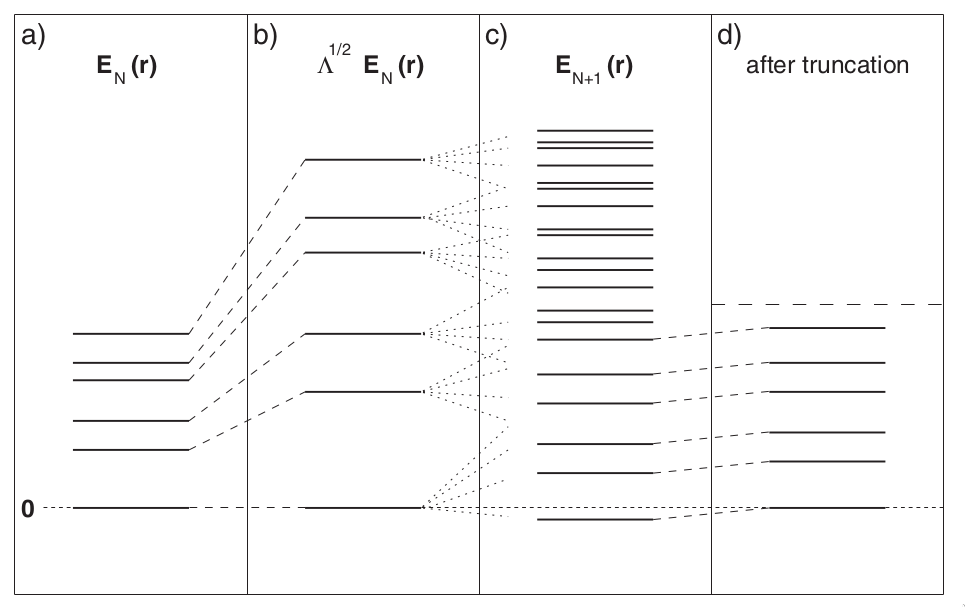
\includegraphics[width=0.6\linewidth]{./gfx/truncation.png}
  \caption{Schematic describing the truncation of states to $N_s$ total states after each iteration.}
  \label{fig:4-nrg-truncation}
\end{figure}


\subsection{Calculation of Thermodynamic Quantities}

Before the setting up of the problem, we briefly present the thermodynamic quantities that we can calculate and compare to those in the literature. The first thing to mention, though, is that since energy and temperature are directly related, each added site corresponds also to an accessing of lower \textit{temperatures}. Via our scaling of the Hamiltonians and the definition of the Boltzmann factors, we have something that looks like

\begin{equation}
  k_B T_N = \frac{1}{2}(1 + \Lambda^{-1})\Lambda^{-(N-1)/2} / \beta.
\end{equation}

For some iteration $N$, we therefore have a relation for the temperature $T_N$ for that iteration. To actually make this determination, we \textit{choose} a value of $\beta$, then plug in $\Lambda$ and $N$ to get $T_N$. Intuitively, a high value of $\beta$ corresponds to low temperatures and a low value of $\beta$ corresponds to high temperatures. We cannot choose too high a value for $\beta$ since this would involve higher temperature effects which we are deliberately truncating after each iteration. On the other hand, we cannot choose too low a value, since we simply wouldn't have enough states/temperatures to perform a valid calculation. It turns out that a value $\sim\mathcal{O}(1)$ is suitable, in particular $0.5$ to 1, or sometimes up to $\sqrt{\Lambda}$, since we take $\Lambda$ to be no greater than 3. With this choice, we are then able to determine $T_N$ and thermodynamic quantities. We took it to be 1.0 in our code.

In particular, we are interested in calculating the entropy $S$, the heat capacity $C$, and the magnetic susceptibility $\chi$:

\begin{align}
  S &= \beta\braket{H} + \ln Z, \\
  C &= \beta^2(\braket{H^2} - \braket{H}^2), \\
  \chi &= \beta(\braket{S_{\mathrm{tot},z}^2} - \braket{S_{\mathrm{tot},z}}^2),
\end{align}

where, as standard in thermodynamics, the average of a quantity $X$ is given by

\begin{equation}
  \braket{X} = \frac{1}{Z}\sum_i X_i e^{-\beta X_i},
\end{equation}

with $Z$ being the partition function. We also note that our goal is to determine the impact the impurity has on these values for a system. In order to do this, we calculate these quantities with the chain in which the impurity is placed at the beginning, as has been described, then we do the same calculates for the chain without the impurity. We subtract off the latter from the former, which yields only the effects due to the impurity.


\subsection{Application to the Project}\label{sec:application-to-project}

There are a number of additional formalities to be discussed regarding the diagonalization of the resulting chain Hamiltonians. However, in spirit of the fact that the NRG method described above is already highly specialized to the Anderson model, I feel it best to leave out the rest of those formalities and instead focus on the specifics of constructing the solutions for this project.

One of the first assumptions we can make is to assume particle-hole symmetry, which has the effect of setting occupation energies for the conductions states to zero, thereby eliminating that term from the Hamiltonian altogether. Another assumption we make is to assume a constant hybridization, meaning the factor $\sqrt{\xi_0/\pi} \rightarrow V$. With this, the initial Hamiltonian turns into, after expanding the impurity part:

\begin{equation}
  H_0 = \Lambda^{-1/2} \left[\sum_\sigma \epsilon_f f^\dagger_\sigma f_\sigma + Uf^\dagger_\uparrow f_\uparrow f^\dagger_\downarrow f_\downarrow  + V\sum_\sigma \left( f^\dagger_\sigma c_{0\sigma} + c^\dagger_{0\sigma}f_\sigma \right)\right],
\end{equation}

and our recursion relation becomes:

\begin{equation}
  H_{N+1} = \sqrt{\Lambda}H_N  + \Lambda^{N/2}\sum_\sigma t_N\left( c^\dagger_{N\sigma}c_{N+1\sigma} + c^\dagger_{N+1\sigma}c_{N\sigma} \right),
\end{equation}


\subsection{Initial Iteration}

With this, we can begin concretely defining our basis and subsequently the actual form of our matrices so that we can diagonalize. Our choice of basis is a set of four states: empty, singly occupied with either spin up or spin down, and doubly occupied. These are denoted with $\ket{0}$, $\ket{\uparrow}$, $\ket{\downarrow}$, $\ket{\uparrow\downarrow}$ respectively. At this point, then, noticing that the impurity Hamiltonian is already diagonal, we can simply write:

\begin{equation}
  \hat{H}_{\mathrm{imp}} = \begin{pmatrix}0 & 0 & 0 & 0 \\ 0 & \epsilon_f & 0 & 0 \\ 0 & 0 & \epsilon_f & 0 \\ 0 & 0 & 0 & 2\epsilon_f + U\end{pmatrix}.\label{eq:4-nrg-himp}
\end{equation}

What this is physically saying is that the unoccupied state has 0 energy, each singly occupied state has energy $\epsilon_f$, and the doubly occupied state has energy $2\epsilon_f$ (one for each electron) plus the Coulomb interaction term $U$.

Now, in the construction of the total Hamiltonian when adding the first site, we consider that the new total basis is a direct/Kronecker product of the original state (that being the impurity for the first iteration) with that of the new site. In general, for some iteration $N$, can denote its basis by $\ket{r}_N$, and the basis of the new site as $\ket{s}_{N+1}$; with this, the new basis is therefore denoted as $\ket{r;s}_{N+1} \equiv \ket{r}_N \otimes \ket{s}_{N+1}$. This is shown in Fig.~\ref{fig:4-nrg-directprod}.

\begin{figure}
  \centering
  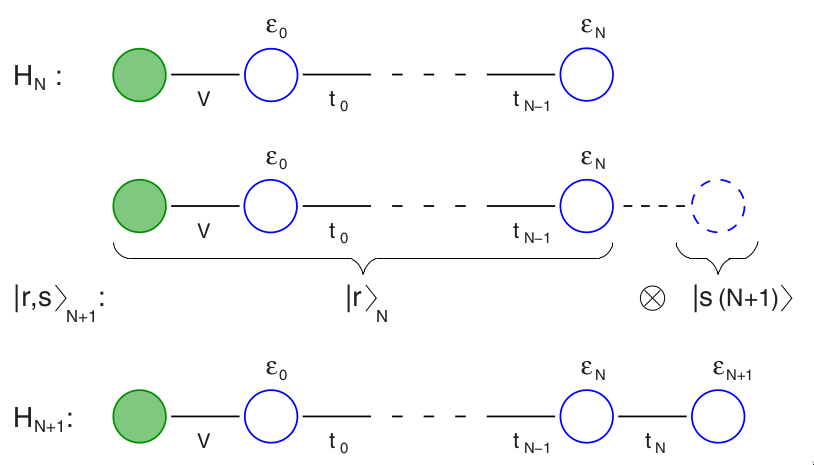
\includegraphics[width=0.6\linewidth]{./gfx/outer-product.png}
  \caption{Schematic of the addition of a site to the end of the chain.}
  \label{fig:4-nrg-directprod}
\end{figure}

In general, for the total Hamiltonian, we have that

\begin{equation}
  \hat{H}_{\mathrm{tot}} = I_4 \otimes \hat{H}_{\mathrm{imp}} + \hat{H}_{c0} \otimes I_4 + \hat{H}_{\mathrm{hyb}},
\end{equation}

where, since we are taking occupation energy of the conduction states to zero, we are left with just:

\begin{equation}
  \hat{H}_{\mathrm{tot}} = I_4 \otimes \hat{H}_{\mathrm{imp}} + \hat{H}_{\mathrm{hyb}},
\end{equation}

with

\begin{equation}
  \hat{H}_{\mathrm{hyb}} = V\sum_\sigma (c^\dagger_{0,\sigma} \otimes f_{\sigma} + c_{0,\sigma} \otimes f^\dagger_{\sigma}).
\end{equation}

It is important to note the order in which the direct product is taken -- for some spaces $A$ and $B$, the form of the new space formed by the direct product $A \otimes B$ will look different than the space formed by the direct product $B \otimes A$. Of course, by switching the order of direct products of operators acting in the total space, one will get back the same results; the spaces aren't \textit{fundamentally} changed by this, they just will \textit{look} different.

Here, we take the first/left space in the direct product to be the conduction site, and each new conduction site will be on the left of the direct product. In principle the definition can be whatever the author would like, but by doing it this way we use the convention that, roughly speaking, the space on the left of the direct product is the ``outer'' or ``larger'' space.

To see this a bit easier, we consider the impurity site and a single conduction site, which is our first iteration. Both spaces have dimensionality of 4, leaving a $16\times16$ matrix. However, we can write it in terms of $4\times4$ block matrices. Here is where the difference between the outer and inner spaces lie: each block itself, being a $4\times4$ matrix, acts on the \textit{inner} space. What this means is that supplanting a $4\times4$ matrix with some non-trival (i.e. not an identity) structure into the main one will have that matrix act on the inner space. Supplanting  \textit{numbers} into the main matrix, i.e. treating the main outer $4\times4$ matrix itself a matrix, corresponds to placing identities at those locations which is trivial in the inner space but has the effect of the main outer $4\times4$ acting on the outer space.\footnote{My understanding of these abstract math concepts is \textit{very} rudimentary; this is certainly not be a mathematically correct way of saying it, but it is \textit{correct} nonetheless, and hopefully helps give a picture of what is going on.}

With this in mind, we can go ahead and construct what the $f$ matrices look like in general (the $c$ matrices will look identical):

\begin{equation}
  f^\dagger_\uparrow = \begin{pmatrix}0 & 0 & 0 & 0 \\ 1 & 0 & 0 & 0 \\ 0 & 0 & 0 & 0 \\ 0 & 0 & -1 & 0\end{pmatrix},\quad f^\dagger_\downarrow = \begin{pmatrix}0 & 0 & 0 & 0 \\ 0 & 0 & 0 & 0 \\ 1 & 0 & 0 & 0 \\ 0 & 1 & 0 & 0\end{pmatrix},
\end{equation}

where the $-1$ is incurred in the construction of $f^\dagger_\downarrow$ due to the matrices' fermionic nature. Referring to our discussion a few paragraphs above, we have that the space for our first iteration is chosen such that the conduction site is the ``outer'' space, meaning, as a 4$\times$4 matrix, each block acts on the impurity space and the main 4$\times$4 matrix acts on the outer space. We present the form of the total Hamiltonian here:

\begin{equation}
  \hat{H}_{\mathrm{tot},0} =
  \begin{pmatrix}
    \mathcal{H}_{\mathrm{imp}} & Vf^\dagger_\uparrow & Vf^\dagger_\downarrow & 0 \\
    Vf_\uparrow & \mathcal{H}_{\mathrm{imp}} & 0 & Vf^\dagger_\downarrow \\
    Vf_\downarrow & 0 & \mathcal{H}_{\mathrm{imp}} & -Vf^\dagger_\uparrow \\
    0 & Vf_\downarrow & -Vf_\uparrow & \mathcal{H}_{\mathrm{imp}}
  \end{pmatrix}.
  \label{eq:4-nrg-htot0}
\end{equation}

The diagonal elements, since they need to act on the impurity space, are themselves matrices; $\mathcal{H}_{\mathrm{imp}}$ is given in Eq.~\eqref{eq:4-nrg-himp}. Additionally, the $f$s are matrices and therefore act on the impurity space. But, we notice $V$s placed in the same places in the main Hamiltonian as in the general form of the $f$s. This corresponds to the $c$ matrices acting on the conduction electron space; with them being placed in the same locations, multipled by $V$, we retrieve the hybrization terms.

\subsection{Symmetry Considerations}


As is customary in physics, we want to consider what symmetries are present in the model in an attempt to reduce the number of things we have to compute, or in this case, reduce the dimensionality of the Hamiltonian. Wilson~\cite{Wilson_1975} chose three good quantum numbers: twice the $z$-component of spin $2S_z$ (the factor of 2 to avoid halfs), the total spin $S$, and the charge $Q$, defined as the particle number with respect to half-filling. This means that $\hat{Q}\ket{0} = -1$, $\hat{Q}\ket{\uparrow} = \hat{Q}\ket{\downarrow} = 0$, and $\hat{Q}\ket{\uparrow\downarrow} = 1$. Considering all three of these symmetries greatly reduced the dimensionality of the problem, and essentially each iteration boiled down to diagonalizing a set of smaller matrices corresponding to the states that share the same set of quantum numbers.

In practice, the inclusion of the total spin as a good quantum number involved the Clebsch-Gordan coefficients, which made things a bit of a mess. Nowadays, computers are good enough that we can compute sufficient iterations quick enough using only $2S_z$ and $Q$, avoiding further complication, and this is what most modern literature uses when discussing NRG, so it is what I will use. Additionally, in the literature, only $S_z$ is written and it is understood that the actual quantity is \textit{twice} $S_z$.

Now, from basic quantum mechanics, we know that if an operator commutes with the Hamiltonian, it shares an eigenbasis. If we construct a new operator using $S_z$ and $Q$ such that it essentially encodes both into one, call this new operator $\hat{Y}$, we are able to write

\begin{align}
  \hat{Y}\hat{H}\ket{\psi} &= E(\hat{Y}\ket{\psi}) \\
  \hat{H}(\hat{Y}\ket{\psi}) &= E(\hat{Y}\ket{\psi}) \\ 
                             &= E\left( \sum_i y_i \ket{Y}_i \right),
\end{align}

where $y_i$ are the eigenvalues and $\ket{Y}_i$ are the eigenstates. The purpose of doing it this way is that many states share the same $S_z$ and $Q$, and hence $y$, meaning two things: the sum over $i$ is effectively less than the original dimensionality of $\hat{H}$, and since our goal is to determine the energy values, we need only diagonalize the resultant block matrices created for the states that share the same $y$. For example, in the first iteration consisting of the $16\times16$ matrix, using this method we reduce the single diagonalization of the $16\times16$ into a few trivial $1\times1$ matrices, four $2\times2$s, and one $4\times4$, which is already a huge improvement; for higher dimensionality matrices, this method becomes incredibly effective.

After doing this and obtaining a series of eigenvalues, we then sort them (and their corresponding states) from smallest to largest, then shift them such that the ground state has an energy of zero. We do this so that we can easily truncate the states corresponding to higher energies/temperatures. Since we are changing the order of the states in our basis, we must also change the $f$ and $c$ matrices to match this. This is done by simply doing:

\begin{equation}
  c_{0,\sigma} \rightarrow \vv{Y}^T c_{0,\sigma} \vv{Y},
\end{equation}

where $Y$ is the matrix of ordered eigenvectors. Lastly, we compute the thermodynamic quantities for this iteration, and continue on to the next.


\subsection{Subsequent Iterations}

The first iteration was special since it involved the impurity hybridizing with the first conduction site. However, after that, subsequent additions of impurity sites is an identical procedure, so the entire rest of the program can be placed inside a loop at this point. Further, these steps are nearly identical to the initial iteration, with a few key differences, that being the dimensionality of the matrices we are constructing, and the inclusion of the hopping terms. We have already described in detail the construction of the block matrices and hence the total Hamiltonian for a given iteration in terms of the different subspaces. We know the form of all the moving pieces, so it should be relatively clear how to generalize this to any subsequent iteration. In principle, the only change is to replaces $V$s with $t$s in Eq.~\eqref{eq:4-nrg-htot0}, and make $\mathcal{H}_{\mathrm{imp}}$ be a larger matrix with the new ordered energies down the diagonal. The $f$s, which turn into the $c$s have the same form but are just larger.










%%% Local Variables:
%%% mode: LaTeX
%%% TeX-master: "../project"
%%% End:
